% Chapter 1

\chapter{Tracking Patterns and Customer Behavior Analysis} % Main chapter title

\label{Chapter1} % For referencing the chapter elsewhere, use \ref{Chapter1} 

\lhead{Chapter 6. \emph{Tracking Patterns and Customer Behavior Analysis}} % This is for the header on each page - perhaps a shortened title

%----------------------------------------------------------------------------------------

\section{Creating Time-Series Data:}

 Time-series data is integral for tracking patterns and analyzing customer behavior evolution due to its ability to capture temporal nuances. By observing changes over time, businesses can uncover seasonal variations, identify trends, and forecast future behavior. This data-driven approach facilitates the detection of anomalies, adaptation of marketing strategies, and segmentation of customers based on temporal patterns. Utilizing time-series analysis improves decision-making, allowing businesses to make informed choices, allocate resources efficiently, and implement targeted campaigns, ultimately optimizing their strategies for dynamic customer preferences and market fluctuations.
\newline
 Hence, I utilized out existing ‘Date’ and ‘Time’ columns to create a ‘Timestamp’ feature for our dataset, which is evidently quite beneficial when conducting time-series analysis:


 % MAKE BLACK AND WHITE 
\begin{table}[htbp]
    \centering
    \rowcolors{1}{blue!20}{white}
    \begin{tabular}{|c|}
        \hline
        \rowcolor{blue!70}
        \textcolor{white}{\textbf{Timestamp Column:}} \\
        \hline
        \rowcolor{blue!50}
        0   2019-01-05 13:08:00\\
        1   2019-03-08 10:29:00 \\
        \rowcolor{blue!50}
        2   2019-03-03 13:23:00 \\
        3   2019-01-27 20:33:00 \\
        \rowcolor{blue!50}
        4   2019-02-08 10:37:00\\
        \hline
    \end{tabular}
    % \caption{Single-column table with alternating blue colors and a header}
    \label{tab:blue_table_with_header}
\end{table}

%----------------------------------------------------------------------------------------
\newpage
\section{Visualizations: }

\begin{figure}[h]
    \centering
    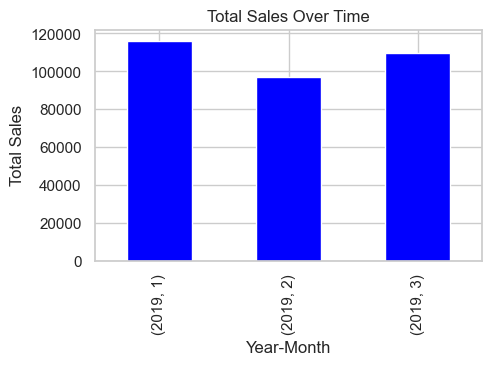
\includegraphics[width=0.7\textwidth]{Chapters/ch6/ch_6_bargraph_2.png}
    % \caption{Radar graph}
    % \label{fig:example}
\end{figure}
This chart depicts the total sales by year-month. As can be seen, February 2019 saw a fall in sales between January and March.
\newline 
\newline 
\begin{figure}[h]
    \centering
    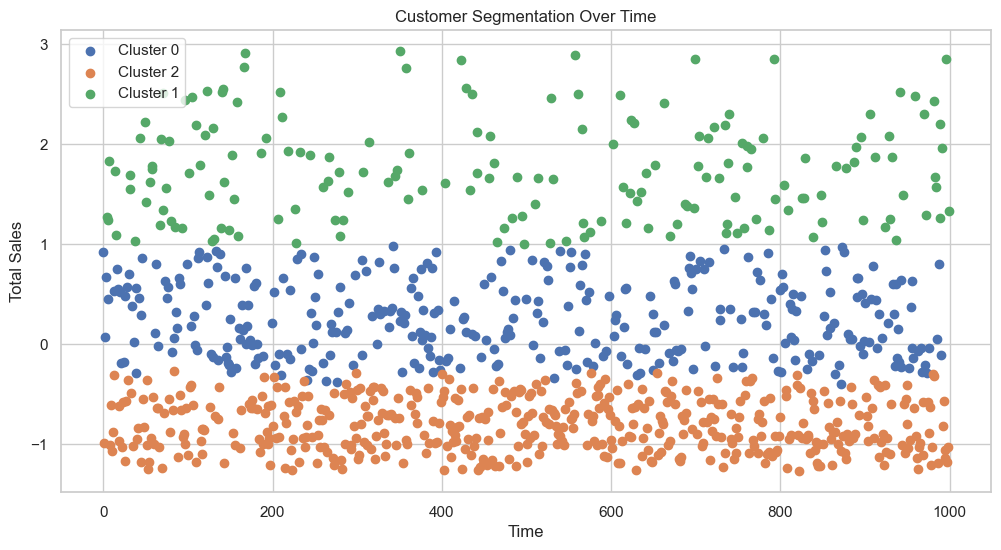
\includegraphics[width=0.7\textwidth]{Chapters/ch6/ch_6_scatterplot.png}
    % \caption{Radar graph}
    % \label{fig:example}
\end{figure}

Using clustering, I was able to visualize customer segmentation over time.

\newpage 
\subsection{Seasonal Decompose Graphs:}

\begin{figure}[h]
    \centering
    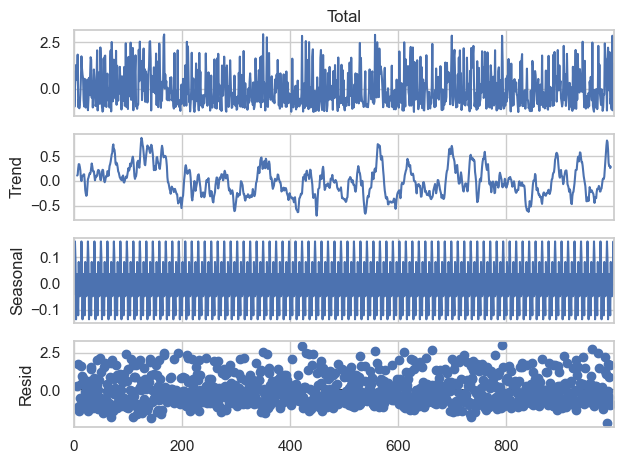
\includegraphics[width=0.7\textwidth]{Chapters/ch6/ch_6_decompose_graph.png}
    % \caption{Radar graph}
    % \label{fig:example}
\end{figure}

Using the \verb|seasonal_decompose| function from statsmodels.tsa, I decomposed a time series into three components: trend, seasonality, and residual. The model is set to 'additive', which means the components are added together. The period is set to 12, indicating a seasonal pattern with a period of 12-time units. 

\begin{itemize}
    \item Observed Component (First Graph): 
    \newline 
    The top scatter plot represents the original time series, which is the observed component. 
As can be seen in the plot, the dense values with high variance suggest that the original time series has fluctuations, noise, or irregular patterns.
    
    \item Trend Component (Second Graph):
    \newline 
    Sets a minimum threshold for the chosen metric. Rules with a confidence value above this threshold will be considered.

    \item Seasonal Component (Third Graph):
    \newline 
    This graph captures the periodic patterns or seasonality in the data, showing how the data varies with a fixed interval (e.g., season). 

    \item Residual Component (Fourth Graph):
    \newline
    This represents the remaining variability after removing the trend and seasonal components. It's essentially the difference between the observed data and the predicted values from the trend and seasonal components. The dense scatter plot suggests that the residuals still contain some variability or noise that is not explained by the trend and seasonal components.
    
\end{itemize}



\subsection{Predictive Modeling using ARIMA: }
ARIMA stands for AutoRegressive Integrated Moving Average. It is a popular time series forecasting model that combines three components: AutoRegressive (AR), Integrated (I), and Moving Average (MA).

\subsubsection{How is it beneficial here? }
ARIMA helps identify and model patterns in the time series data, including seasonality, trends, and cyclical behaviors. It captures historical patterns to make predictions about future values.
\newline 
\newline 
Forecasting Customer Behavior: By applying ARIMA to historical customer behavior data (e.g., sales over time), the model can provide forecasts for future behavior. This can be valuable for planning marketing strategies, inventory management, and overall business decision-making.
\newline 
\newline 
Understanding Trends: The trend component of the ARIMA model helps in understanding the overall direction of the time series. This can be useful in identifying long-term trends in customer behavior.
\newline 
\newline 
ARIMA models, however, assume that the underlying patterns in the data are linear and stationary. For more complex and dynamic patterns, other time series models or machine learning approaches may be considered.


\subsubsection{Applying the model:}
ARIMA(df5['Total'], order=(1, 1, 1)): This initializes an ARIMA model using the ARIMA class.
order=(1, 1, 1) specifies the order of the ARIMA model. Here, (1, 1, 1) means:

\begin{itemize}
    \item p=1: One autoregressive term. It models the relationship between the current value and its immediate previous value (lag 1).
    
    \item d=1: One differencing. It indicates that the time series is differenced once to achieve stationarity. Differencing involves subtracting the previous value from the current value.

    \item q=1: One moving average term. It models the dependency between the current value and the residual error from the lagged moving average terms.
\end{itemize}

model.fit(): This fits the ARIMA model to the provided time series data (df5['Total']).
\verb|result.get_forecast(steps=forecast_steps)|: This generates forecasts for the next \verb|forecast_steps| time points using the fitted ARIMA model.
\verb|predicted_mean|: This extracts the predicted mean values from the forecast result. The mean values represent the point estimates of the forecast.


\subsubsection{Prediction and analysis}

\begin{figure}[h]
    \centering
    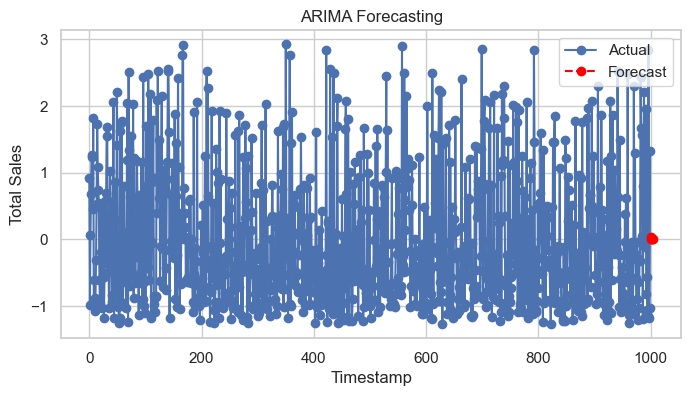
\includegraphics[width=0.7\textwidth]{Chapters/ch6/ch_6_pred_and_analysis.png}
    % \caption{Radar graph}
    % \label{fig:example}
\end{figure}

The dense distribution of blue points represents the actual "Total" sales values over time. The constant variation suggests that the sales data exhibit fluctuations or variability.
\newline 

The sparse presence of red points (forecast) at the end of the x-axis indicates the predicted "Total" sales values for the next 5 time points. The small size of the red dots suggests that the model is forecasting relatively low variations or changes in sales over this short-term forecast horizon. Hence, there seems to be a relatively stable or slowly changing trend in future sales.
\newline 
% \newline 
The sparse and concentrated nature of the red points might also suggest a high level of confidence in the forecast, as the model is projecting a narrow range of potential outcomes.
\newline 
% \newline
From all this we may conclude that there won’t be much change in customer behavior soon.

\subsection{Feature Engineering to calculate and visualize Rolling Mean:}
\newpage 
\subsubsection{The visualization:}
\begin{figure}[h]
    \centering
    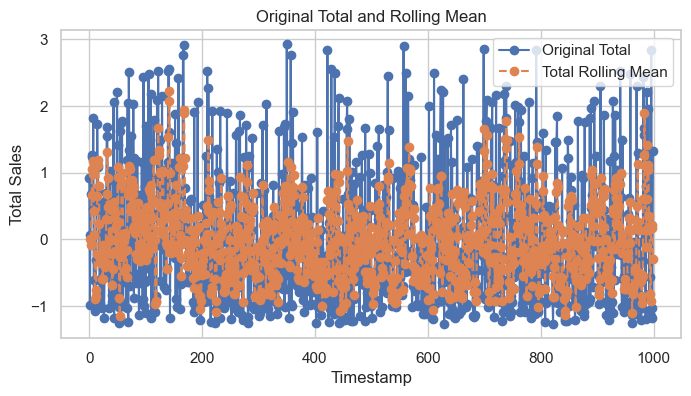
\includegraphics[width=0.7\textwidth]{Chapters/ch6/ch_6_rolling_mean.png}
    % \caption{Radar graph}
    % \label{fig:example}
\end{figure}

\subsubsection{How the graph works: }
The purpose of calculating the rolling mean is to smooth out short-term fluctuations or noise in your data and highlight longer-term trends. In this case, we are using it to provide a clearer picture of how the "Total" sales values are evolving over time. We’re using a rolling window of size 3. A rolling window refers to a fixed-size subset of consecutive data points that "rolls" or moves through the dataset as you analyze it. This helps in revealing trends and patterns.

\subsubsection{Analyzing the visualization}
The dense blue (Original Total) that can be seen throughout the graph, indicates frequent fluctuations or variations in the sales values. This could be due to regular transactions or short-term patterns in customer behavior. \newline 
In contrast, the orange points (Total Rolling Mean) are denser at the bottom half of the chart. Thus, the rolling mean is consistently lower than the actual sales value. This represents a downward trend or a smoothing effect that levels out short-term spikes or peaks in the original data. Hence, there are periods of lower sales that are being averaged out.
\newline 
Based on all this, we can conclude that there are frequent fluctuations in total sales, which are potentially being influenced by daily transactions or short-term trends. 

%----------------------------------------------------------------------------------------
